\chapter{Distribution Analysis} \label{sec: disanalysis}

\section{Normalized Distributions}

As mentioned in section \ref{sec:definitions}, the variables $H_{T}$ and $S_{T}$ were defined to achieve a greater separation between background and signal. Figures \ref{fig: HTunitNC} and \ref{fig: STunitNC} show normalized to the unity plots with no additional cuts in the variables. The plots in both figures show that a separation between signal and background is achieved for values greater than 500 GeV for both $H_{T}$ and $S_{T}$.

The plot shown in Figure \ref{fig: tau1pTunitNC} shows the distribution for the transverse momentum of the main $\tau$. It can be seen that the shape of the signal distribution separates from the backgrounds at around 150 GeV.

\begin{figure}
\centering
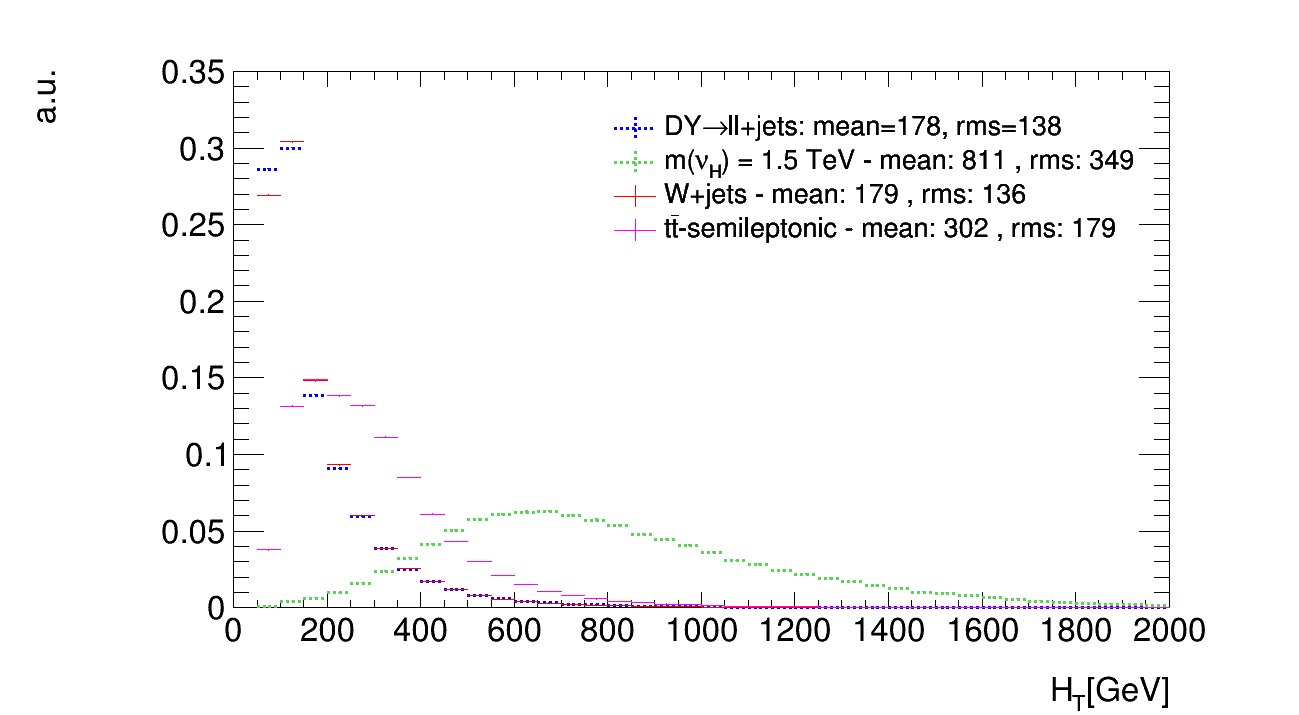
\includegraphics[width=1.2\linewidth]{Figures/Plots/HT_unitNoCuts}
\caption{Unit plot of $H_{T}$ with no cuts}
\label{fig: HTunitNC}
\end{figure}

\begin{figure}
\centering
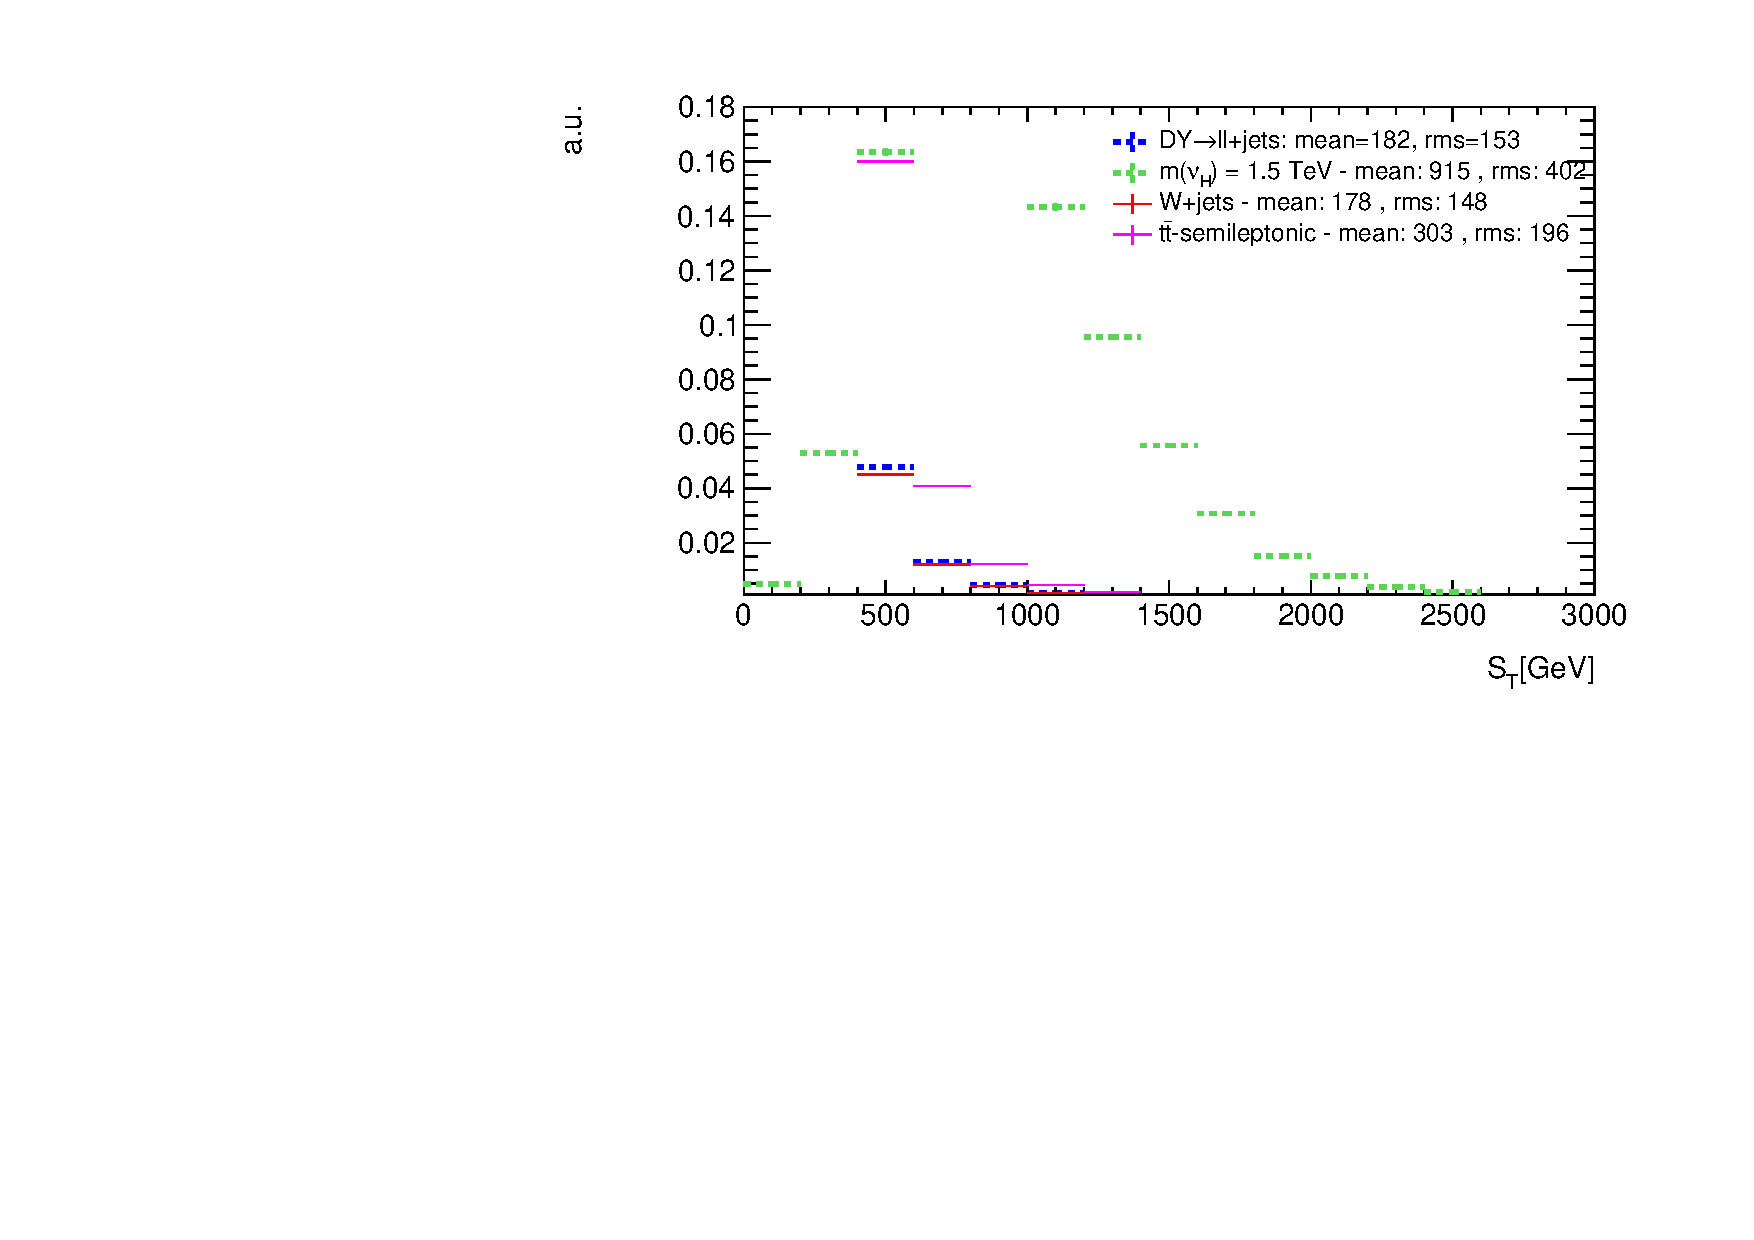
\includegraphics[width=1.2\linewidth]{Figures/Plots/ST_unitNoCuts}
\caption{Unit plot of $S_{T}$ with no cuts}
\label{fig: STunitNC}
\end{figure}

\begin{figure}[H]
\centering
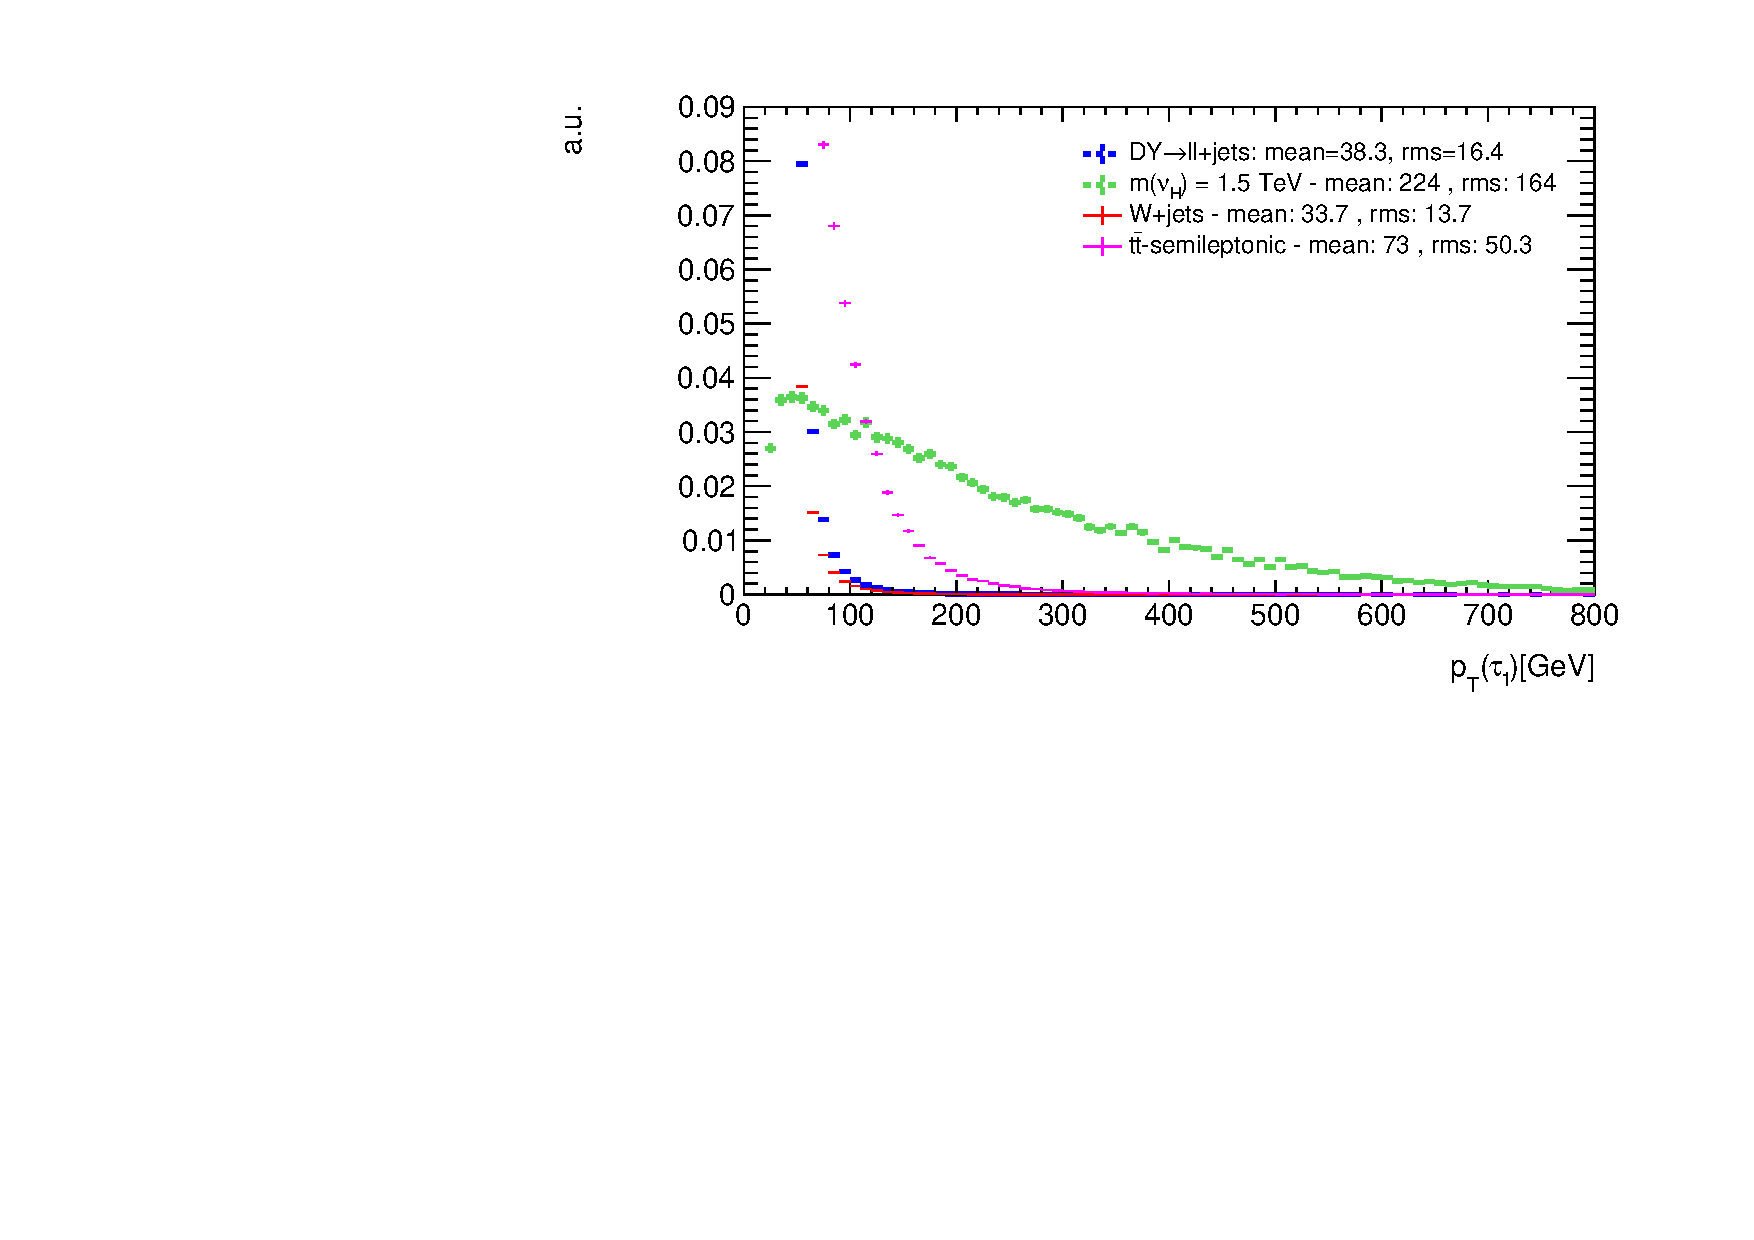
\includegraphics[width=1.2\linewidth]{Figures/Plots/tau1_pT_unitNoCuts}
\caption{Unit plot of $p_{T}$ from the leading $\tau$ with no cuts}
\label{fig: tau1pTunitNC}
\end{figure}
